\documentclass{beamer}
\usepackage[utf8]{inputenc}

\usepackage{color}
\usepackage{xcolor}
\definecolor{PLB}{rgb}{0.06,0.42,0.60}
\definecolor{PLBfonce}{rgb}{0.06,0.42,0.60}
\definecolor{PLBmoyen}{RGB}{176, 216, 232}
\definecolor{PLBpale}{rgb}{0.94,0.965,0.965}

%\usetheme{PaloAlto}
\usetheme{Madrid}
\setbeamercolor{frametitle}{bg=PLB}     %controls the color of the headline
\setbeamercolor{sidebar}{bg=PLB}        %controls the color of the sidebar
\setbeamercolor{logo}{bg=PLB!70!black}
\setbeamercolor{structure}{fg=PLB, bg=PLB!40}
%\setbeamertemplate{footline}[default]
\setbeamertemplate{enumerate items}[square]
\setbeamertemplate{itemize items}[circle]

\setbeamerfont{section number projected}{size=\large}
\setbeamertemplate{section in toc}[circle]
\setbeamertemplate{subsection in toc}[square]

\usepackage{amssymb}
\usepackage{pifont}
\usepackage{bigints}
\usepackage{mathrsfs}
\usepackage{physics}

\definecolor{mblue}{rgb}{0.18,0.21,0.67}
\definecolor{mgreen}{rgb}{0.56,0.74,0.}
\definecolor{dgreen}{rgb}{0.,0.6,0.}
\definecolor{violet}{RGB}{142, 68, 173}
\definecolor{bleu}{RGB}{41, 128, 185}
\definecolor{gris}{rgb}{0.5,0.5,0.5}
\newcommand{\cmark}{{\color{dgreen}\ding{52}}}
\newcommand{\xmark}{{\color{red}\ding{55}}}
\newcommand{\bmark}{{\color{orange}$\sim$}}
\newcommand{\arrow}{{\color{PLB}\ding{220}}}
\newcommand{\mbold}[1]{{\textbf{\color{PLB}#1}}}
\newcommand{\I}{\dot{\imath}}

\usepackage{soul}
\usepackage{multicol}
\usepackage{multirow}

\usepackage{ifthen}

\usepackage{amsmath}
\usepackage{cancel}
\DeclareMathOperator*{\argmax}{argmax}
\DeclareMathOperator*{\argmin}{argmin}
\DeclareMathOperator\erfi{erfi}

\usepackage[backend=bibtex, style=authoryear-comp]{biblatex}
\usepackage{filecontents}
\renewbibmacro*{cite}{%
  \iffieldundef{shorthand}
    {\ifthenelse{\ifnameundef{labelname}\OR\iffieldundef{labelyear}}
       {\usebibmacro{cite:label}%
        \setunit{\printdelim{nonameyeardelim}}}
       {\printnames{labelname}%
        \setunit{\printdelim{nameyeardelim}}}%
     \usebibmacro{cite:labeldate+extradate}%
     \setunit{\addcomma\space}%
     \usebibmacro{journal}}
    {\usebibmacro{cite:shorthand}}}
%\newcommand{\customcite}[1]{\citeauthor{#1} (\citeyear{#1})}
\newcommand{\customcite}[1]{\cite{#1}}

\bibliography{biblio}

\beamertemplatenavigationsymbolsempty

\usepackage{bm}
\newcommand{\Mvb}[1]{\boldsymbol{#1}}

%for backup slides
\newcommand{\backupbegin}{
  \newcounter{finalframe}
  \setcounter{finalframe}{\value{framenumber}}
}
\newcommand{\backupend}{
  \setcounter{framenumber}{\value{finalframe}}
}


\AtBeginSection[
  {\frame<beamer>{\frametitle{Outline}   
    \tableofcontents[currentsection,currentsection]}}%
]%
{
  \frame<beamer>{ 
    \frametitle{Outline}   
    \tableofcontents[currentsection,currentsection]}
}

\newenvironment{bframe}[1]% frame of backup (to get bakcup in title) 
{% begin code
  \begin{frame}{{\small\texttt{backup}\ } #1}
}%
{% end code
  \end{frame}
}


%\title[Workshop Bordeaux]{Hybrid model of Vlasov-Maxwell equations\\ and\\ comparison of Hamiltonian method and Lawson method}
\title[]{ (Approximate) Exponential methods for solving hyperbolic problems for electron hybrid model}
\author[Josselin Massot]{A. Crestetto \inst{1} \and N. Crouseilles \inst{2,3} \and Y. Li \inst{4} \and \underline{J. Massot} \inst{3,2}}
\institute[IRMAR]{
       \inst{1} LMJL, Université de Nantes
  \and \inst{2} Inria Rennes -- Bretagne Atlantique
  \and \inst{3} IRMAR, Université de Rennes
  \and \inst{4} Max Planck Institute for Plasma Physics, Garching, Germany
}
\date{October 21, 2021}


\AtBeginDocument{\colorlet{defaultcolor}{.}}

\begin{document}
% -------------------------------------------------------------------
% --- BEGIN DOCUMENT ------------------------------------------------
% -------------------------------------------------------------------

\begin{frame}[plain]
  \titlepage
\end{frame}
\begin{frame}{Outline}
  \tableofcontents
\end{frame}

% -------------------------------------------------------------------
% --- INTRODUCTION --------------------------------------------------
% -------------------------------------------------------------------
\section{Introduction}
\begin{frame}{Introduction}
  A nonlinear transport in $(z,v_x,v_y,v_z)\in\Omega\times\mathbb{R}^3$ of a cold (fluid) electron density distribution (reconstruction from current variable $\Mvb{j}_c$) and a hot (kinetic) electron density distribution $f_h$:
  \begin{thebibliography}{9}
    \setbeamertemplate{bibliography item}[article]
    \bibitem{a} \customcite{Holderied:2020}
  \end{thebibliography}
  $$
    \begin{cases}
      \partial_t\Mvb{j}_c = \Omega_{pe}^2\Mvb{E} - J\Mvb{j}_c B_0 \\
      \partial_t\Mvb{B}   = J\partial_z\Mvb{E} \\
      \partial_t\Mvb{E}   = -J\partial_z\Mvb{B} - \Mvb{j}_c + \int_{\mathbb{R}^3} v_\perp f_h\dd{\Mvb{v}} \\
      \partial_t f_h  + v_z\partial_z f_h - \left( \Mvb{E} + \Mvb{v}\times(\Mvb{B}+\Mvb{B}_0) \right)\cdot\nabla_{\Mvb{v}} f_h = 0
    \end{cases}
  $$
  with:
  $$
    J = \begin{pmatrix}
       0 & 1 \\
      -1 & 0
    \end{pmatrix}
  $$
  \mbold{We want:}
  \begin{itemize}
    \item High order time integrator and space integrator (FFT + WENO)
    \item Efficient adaptive time step method
  \end{itemize}
\end{frame}

% -------------------------------------------------------------------
% --- LAWSON METHOD -------------------------------------------------
% -------------------------------------------------------------------
\section{Numerical method and approximation}

\begin{frame}{Lawson method}
  We would like to solve
  $$
    \partial_t u = Lu + N(t,u)
  $$
  Change of variable: \mbold{$v = e^{-tL}u$}, we obtain:
  $$
    \begin{aligned}
      \dot{v}(t) &= -Le^{-tL}u(t) + e^{-tL}\underbrace{\left(Lu(t) + N(t,u)\right)}_{\dot{u}(t)} \\
                 &= e^{-tL}N(t,e^{tL}v)
    \end{aligned}
  $$
  which can be solve with a \mbold{Runge-Kutta method} in $v$, that can be rewritten in $u$, for example with Euler method:
  $$
    v(t^n+\Delta t) \approx v^{n+1} = v^n + \Delta t e^{-t^nL}N(t^n,e^{t^nL}v^n)
  $$
  or as an expression of $u$:
  $$
    u^{n+1} = e^{\Delta t L}u^n + \Delta te^{\Delta t L}N(t^n,u^n)
  $$
  \begin{thebibliography}{9}
    \setbeamertemplate{bibliography item}[article]
    \bibitem{e} \customcite{Lawson:1967a}
    \bibitem{f} \customcite{Hochbruck:2020}
  \end{thebibliography}
\end{frame}
%-------%
\begin{frame}{Lawson method}
  {Pros \& Cons}
  \begin{description}
    \item[\cmark] Numerically efficient (order increases linearly-ish with the number of stages)
    \item[\cmark] Literature on Runge-Kutta method (embedded-RK, IMEX methods, low storage methods, \dots)
    \item[\cmark] Linear part is solved exactly
    \item[\xmark] Stability constraint (not from the linear part \cmark)
    \item[\xmark] Behavior in long time
    \item[\bmark] Needs to compute (efficiently) $e^{\tau L}$ for any $\tau=c_j\Delta t$ and $L$
  \end{description}
\end{frame}

\begin{frame}{How to compute efficiently $e^{\tau L}$ ?}
  \mbold{Why this could be complicated ?}
  \begin{description}
    \item[\xmark] We would like a formal form depending on time parameter $\tau$ and all hidden parameters of matrix $L$
  \end{description}

  \mbold{Solutions:}
  \begin{description}
    \item[Taylor series:] simplest and first method studing
    \item[Padé approximant:] defined as the best rational approximation of a function
    \item[\dots:] Some other methods don't explor yet
      \vspace{-0.1cm}
      \begin{thebibliography}{9}
        \setbeamertemplate{bibliography item}[article]
        \bibitem{i} \customcite{Moler:2003}
      \end{thebibliography}
  \end{description}

  \mbold{Simplification:}
  \begin{itemize}
    \item Suppose $L$ diagonalizable and all its eigenvalues are pure imaginary $\text{sp}(L)\subset\I\mathbb{R}\implies \text{sp}(e^{tL})\subset\mathcal{C}(0,1)$.
  \end{itemize}
\end{frame}

\begin{frame}{Taylor series}
  Simplest approximation:
  $$
    T_p(\tau L) = \sum_{k=0}^p \frac{\tau^k}{k!}L^k = e^{\tau L} + \order{\tau^{p+1}}
  $$

  \begin{theorem}
    $\text{sp}(L)\subset\I\mathbb{R}\smallsetminus\I[-1,1]$ implies eigenvalues diverge
  \end{theorem}
  \emph{Proof:} compute Taylor series outside of its convergence radius

  \mbold{Conclusion:}
  \begin{description}
    \item[\xmark] Bad behavior of eigenvalues
    \item[\xmark] Numerical instability in scheme
  \end{description}
\end{frame}
\begin{frame}{Eigenvalues of Taylor series}
   \begin{figure}\centering
    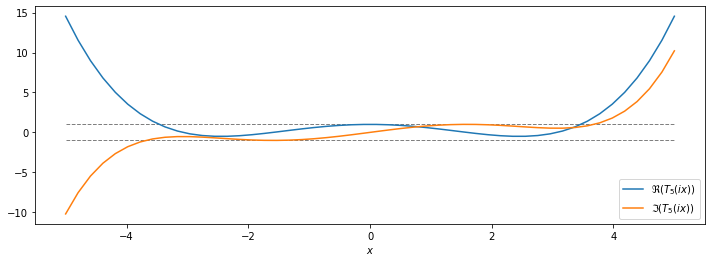
\includegraphics[height=0.35\textheight]{img/T5_reim}
    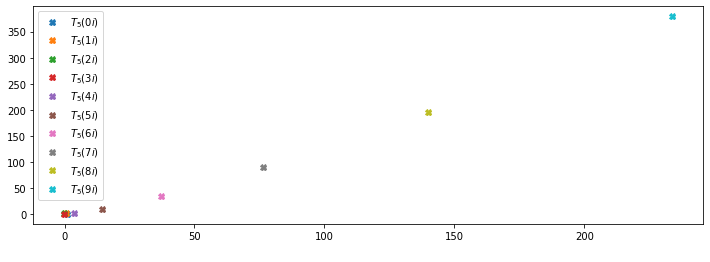
\includegraphics[height=0.35\textheight]{img/T5_ev}
    \caption{$T_5(\I x)$, $x\in[\![0,9]\!]$}
  \end{figure}
\end{frame}

\begin{frame}{Padé approximant}
  Best rational approximation of exponential function. \\
  Defined (for order~$(p,q)$) as:
  $$
      h_{p,q}(M) = \sum_{i=0}^p        \frac{\frac{p!}{(p-i)!}}{\frac{(p+q)!}{(p+q-i)!}} \frac{M^i}{i!} \quad,\quad
      k_{p,q}(M) = \sum_{j=0}^q (-1)^j \frac{\frac{q!}{(q-j)!}}{\frac{(p+q)!}{(p+q-j)!}} \frac{M^j}{j!}
  $$
  Finally Padé approximant is:
  $$
    P_{p,q}(\tau L) = h_{p,q}(\tau L)\left( k_{p,q}(\tau L) \right)^{-1} = e^{\tau L} + \order{\tau^{p+q+1}}
  $$
  \vspace{-0.5cm}
  \begin{theorem}
    $$\text{sp}(L)\subset\I\mathbb{R} \implies \text{sp}(P_{p,p}(tL))\subset\mathcal{C}(0,1)$$
  \end{theorem}

  \mbold{Conclusion:}
  \begin{description}
    \item[\xmark] Needs matrix inversion, or some tricks:
      \vspace{-0.1cm}
      \begin{thebibliography}{9}
        \setbeamertemplate{bibliography item}[article]
        \bibitem{j} \customcite{Li:2011}
      \end{thebibliography}
    \item[\cmark] Best approximation for this numerical cost
    \item[\cmark] Preserve eigenvalues
  \end{description}
\end{frame}
\begin{frame}{\emph{Proof}}
  $L$ diagonalizable and $\text{sp}(L)\subset\I\mathbb{R}$ $\implies$ $L = Q^{-1}DQ$
  $$
    \begin{aligned}
      P_{p,p}(L) &= \left(\sum_{k=0}^p \frac{1}{k!}Q^{-1}D^kQ\right)\cdot\left(\sum_{\ell=0}^p (-1)^\ell\frac{1}{\ell!}Q^{-1}D^\ell Q\right)^{-1}\\
                 &= Q^{-1}\left( \textcolor{violet}{\sum_{k=0}^p \frac{1}{k!}D^k} \right)\cdot\left(\textcolor{dgreen}{\sum_{\ell=0}^p (-1)^\ell\frac{1}{\ell!}D^\ell}\right)^{-1}Q
    \end{aligned}
  $$
  with $D = \text{diag}(\{ \I\alpha_j , j=1,\dots,d\})$
  $$
    \begin{aligned}
      \textcolor{violet}{\sum_{k=0}^p \frac{1}{k!}D^k} &= \text{diag}\!\!\left(\!\!\left\{ \sum_{k=0}^{\lfloor\frac{p}{2}\rfloor} (-1)^k\frac{\alpha_j^{2k}}{{2k}!} \textcolor{red}{\Mvb{+}}\I\!\!\sum_{k=0}^{\lfloor\frac{p}{2}\rfloor-1} (-1)^k \frac{\alpha_j^{2k+1}}{(2k+1)!} , j\in[\![0,d]\!] \right\}\!\!\right) \\
      \textcolor{dgreen}{\sum_{\ell=0}^p (-1)^\ell\frac{1}{\ell!}D^\ell} &= \text{diag}\!\!\left(\!\!\left\{ \sum_{\ell=0}^{\lfloor\frac{p}{2}\rfloor} (-1)^\ell\frac{\alpha_j^{2\ell}}{{2\ell}!} \textcolor{red}{\Mvb{-}}\I\!\!\sum_{\ell=0}^{\lfloor\frac{p}{2}\rfloor-1} (-1)^\ell \frac{\alpha_j^{2\ell+1}}{(2\ell+1)!} , j\in[\![0,d]\!] \right\}\!\!\right)
    \end{aligned}
  $$

  $\textcolor{dgreen}{\lambda^-} = \overline{\textcolor{violet}{\lambda^+}}$ so $\left|\frac{\lambda^+}{\lambda^-}\right|=1$.
\end{frame}

\begin{frame}{Eigenvalues of Padé approximant}
  \begin{figure}\centering
   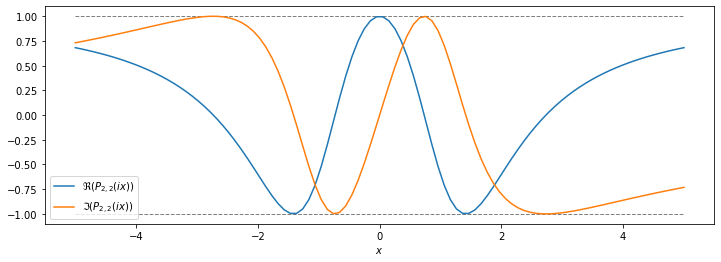
\includegraphics[height=0.35\textheight]{img/P22_reim}
   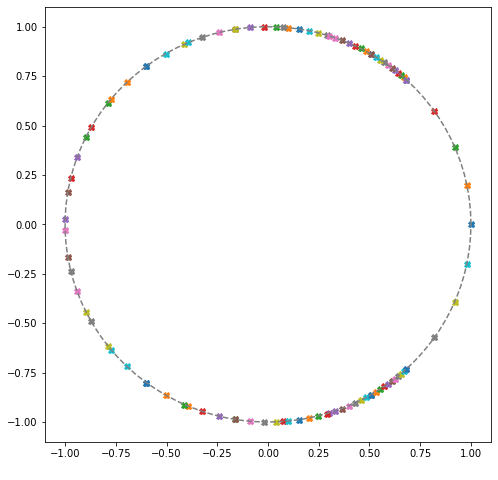
\includegraphics[height=0.35\textheight]{img/P22_ev}
   \caption{$P_{2,2}(\I x)$, $x\in[-5,5]$}
 \end{figure}
\end{frame}

\begin{frame}{Eigenvalues of assymetric Padé approximants}
  \begin{columns}
    \begin{column}{0.5\textwidth}
      \begin{figure}\centering 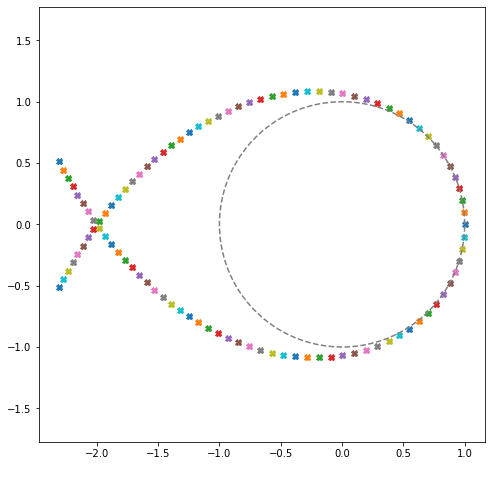
\includegraphics[width=\textwidth]{img/P21_ev} \caption{$P_{2,1}(\I x)$ $x\in[-5,5]$}\end{figure}
    \end{column}
    \begin{column}{0.5\textwidth}
      \begin{figure}\centering 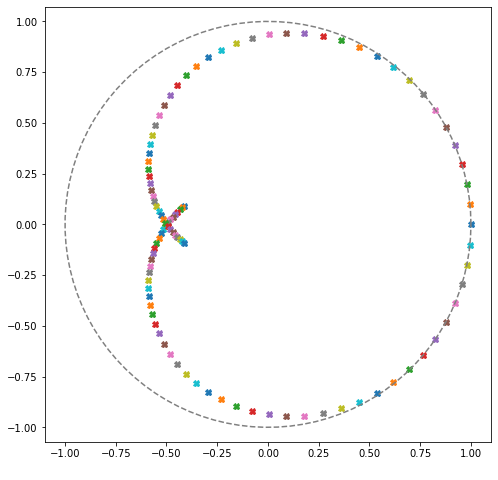
\includegraphics[width=\textwidth]{img/P12_ev} \caption{$P_{1,2}(\I x)$ $x\in[-5,5]$}\end{figure}
    \end{column}
  \end{columns}
\end{frame}

\begin{frame}{Error on approximate Lawson method}
  We note $\mathfrak{exp}(L) = P_{p.q}(L)$ or $T_p(L)$, generic approximation.
  $$\mathfrak{exp}(L) = e^L + \mathcal{O}(L^{r+1})$$

  Lawson RK(3,3) method:
  $$
    \begin{aligned}
      u^{(1)} &= e^{\Delta t L}u^n + \Delta te^{\Delta t L}N(t^n,u^n) \\
      u^{(2)} &= \frac{3}{4}e^{\frac{\Delta t}{2} L}u^n + \frac{1}{4}e^{-\frac{\Delta t}{2} L}u^{(1)} + \frac{\Delta t}{4}e^{-\frac{\Delta t}{2} L} N(t^n+\Delta t,u^{(1)}) \\
      u^{n+1} &= \frac{1}{3}e^{\Delta t L}u^n + \frac{2}{3}e^{\frac{\Delta t}{2} L}u^{(2)} + \frac{2}{3}\Delta t e^{\frac{\Delta t}{2} L} N(t^n+\frac{\Delta t}{2},u^{(2)})
    \end{aligned}
  $$
  \mbold{If} $L$ and $N$ commute: $u^{n+1} = e^{\Delta tL}\left(I + N + \frac{N^2}{2} + \frac{N^3}{6} \right)u^n$, stability is same as RK(3,3). \mbold{Else}\dots
\end{frame}
\begin{frame}{Error on approximate Lawson method}
  \mbold{If} $L$ and $N$ don't commute:
  $$
    \begin{aligned}
      u^{n+1} = \Big[ e^{\Delta tL}
        &+\Delta t\left(\frac{2}{3}e^{\frac{\Delta t}{2}L}Ne^{\frac{\Delta t}{2}L}+\frac{1}{6}e^{\Delta tL}N + \frac{1}{6}Ne^{\Delta tL}\right)
          \textcolor{gris}{\rightsquigarrow e^{\Delta L}\Delta t N} \\
        & + \frac{\Delta t^2}{2}\left(\frac{1}{3}Ne^{\Delta tL}N + \frac{1}{3}e^{\frac{\Delta t}{2}L}Ne^{\frac{\Delta t}{2}L}N + \frac{1}{3} e^{\frac{\Delta t}{2}L}Ne^{-\frac{\Delta t}{2}L}Ne^{\Delta tL} \right) \\
          &\hspace{2cm} \textcolor{gris}{\rightsquigarrow e^{\Delta L}\frac{\left(\Delta t N\right)^2}{2}} \\
      & + \frac{\Delta t^3}{6}e^{\frac{\Delta t}{2}L}Ne^{-\frac{\Delta t}{2}L}Ne^{\Delta tL}N \Big]u^n \textcolor{gris}{\rightsquigarrow e^{\Delta L}\frac{\left(\Delta t N\right)^3}{6}}
    \end{aligned}
  $$
  Same results if $e^{\Delta t L}\mapsto \mathfrak{exp}(\Delta t L) = e^{\Delta t L} + \mathcal{O}(\Delta t^{r+1})$

  \begin{lemma}
    Error for Lawson RK($m$,$s$) is always in $\mathcal{O}(\Delta t^{m+1})+\mathcal{O}(\Delta t^{r+1})$
  \end{lemma}
\end{frame}

% -------------------------------------------------------------------
% --- NUMERICAL TESTS -----------------------------------------------
% -------------------------------------------------------------------
\section{Numerical tests}
\begin{frame}{Test 1}{2D translation test case}
  $$\partial_t u + a\partial_x u + b\partial_y u = 0$$
  
  After a Fourier transform in $y$
  $$
    \partial_t \hat{u}
      + \underbrace{\I bk\hat{u}}_{L \hat{u}}
      + \underbrace{\widehat{a\partial_x u}}_{N(\hat{u})}
      = 0
  $$

  First test with:
  \begin{itemize}
    \item Lawson RK(3,3) method
    \item Lawson RK(3,3) method with Taylor series $T_p$, $p\in[\![1,4]\!]$
    \item Lawson RK(3,3) method with Padé approximant $P_{p,q}$, $p,q \in[\![1,2]\!]$
  \end{itemize}
  \mbold{Mesure order:} $x,y\in[-2,2]$, $N_x=N_y=243$, $a=1.0$, $b=0.75$, $T_f=0.07111$, $\Delta t\in[0.00158,0.02370]$.
\end{frame}
\begin{frame}{Test 1}{2D translation test case: mesure of order}
  \only<1>{
    \begin{figure}
      \centering
      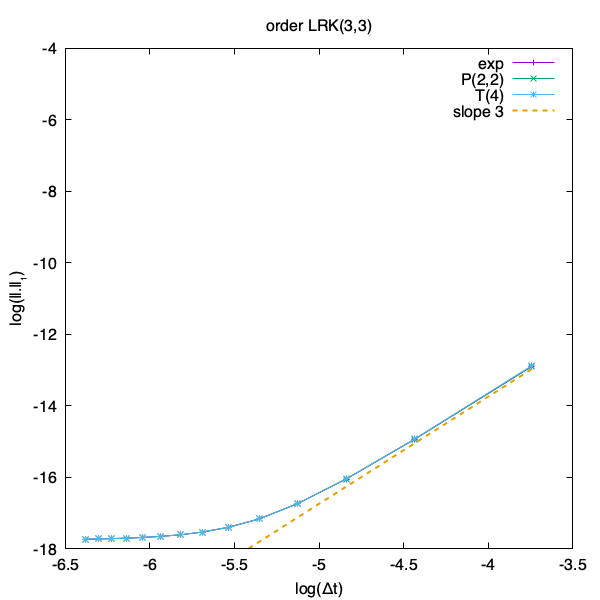
\includegraphics[height=0.6\textheight]{img/order_lrk33ref}
      \caption{Order of Lawson RK(3,3) method, and Lawson RK(3,3), $P_{2,2}$ approximant method and Lawson RK(3,3) $T_4$ series method.}
    \end{figure}
  }\only<2>{
    \begin{columns}
      \begin{column}{0.5\textwidth}
        \begin{figure}
          \centering
          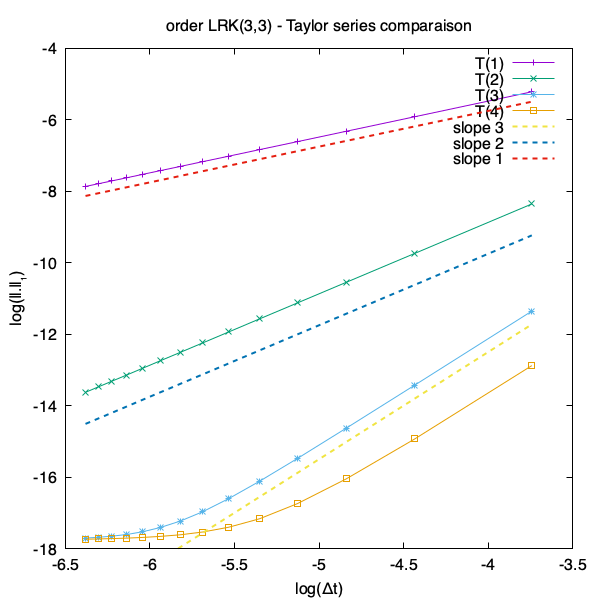
\includegraphics[height=0.6\textheight]{img/order_lrk33taylor}
          \caption{Order of Lawson RK(3,3) $T_p$ series method, $p=1,\dots,4$.}
        \end{figure}
      \end{column}
      \begin{column}{0.5\textwidth}
        \begin{figure}
          \centering
          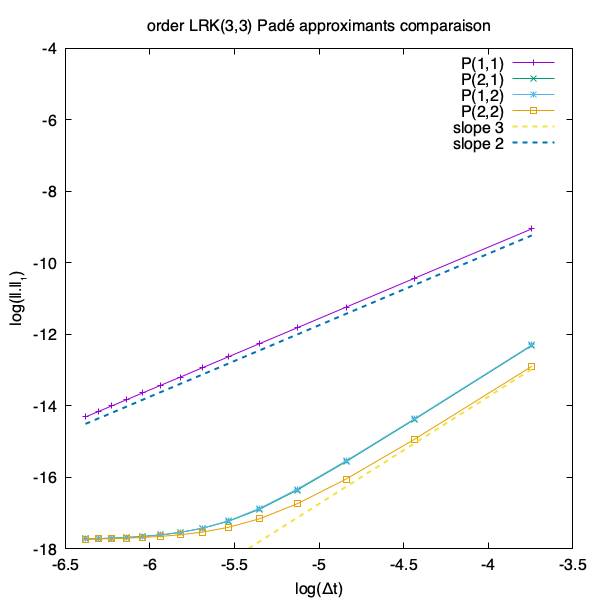
\includegraphics[height=0.6\textheight]{img/order_lrk33pade}
          \caption{Order of Lawson RK(3,3) $P_{p,q}$ approximant, $p=1,2$, $q=1,2$}
        \end{figure}
      \end{column}
    \end{columns}
  }
\end{frame}

\begin{frame}{Test 2}{2D rotation test case}
  $$\partial_t u - y\partial_x u + x\partial_y u = 0$$

  After a Fourier transform in $y$
  $$\partial_t \hat{u} + \underbrace{\I xk\hat{u}}_{L \hat{u}} + \underbrace{\widehat{-y\partial_x u}}_{N(\hat{u})} = 0$$

  Second test with same methods:
  \begin{itemize}
    \item Lawson RK(3,3) method
    \item Lawson RK(3,3) method with Taylor series $T_3$, $p=3$
    \item Lawson RK(3,3) method with Padé approximant $P_{1,1}$, $p=q1$
  \end{itemize}
  \mbold{Test Taylor instability:} $x,y\in[-2,2]$, $N_x=N_y=81$, $T_f=1.52891$, $\Delta t=0.020944$.
\end{frame}
\begin{frame}{Test 2}{2D rotation test case: test Taylor series instability}
  \begin{figure}
    \centering
    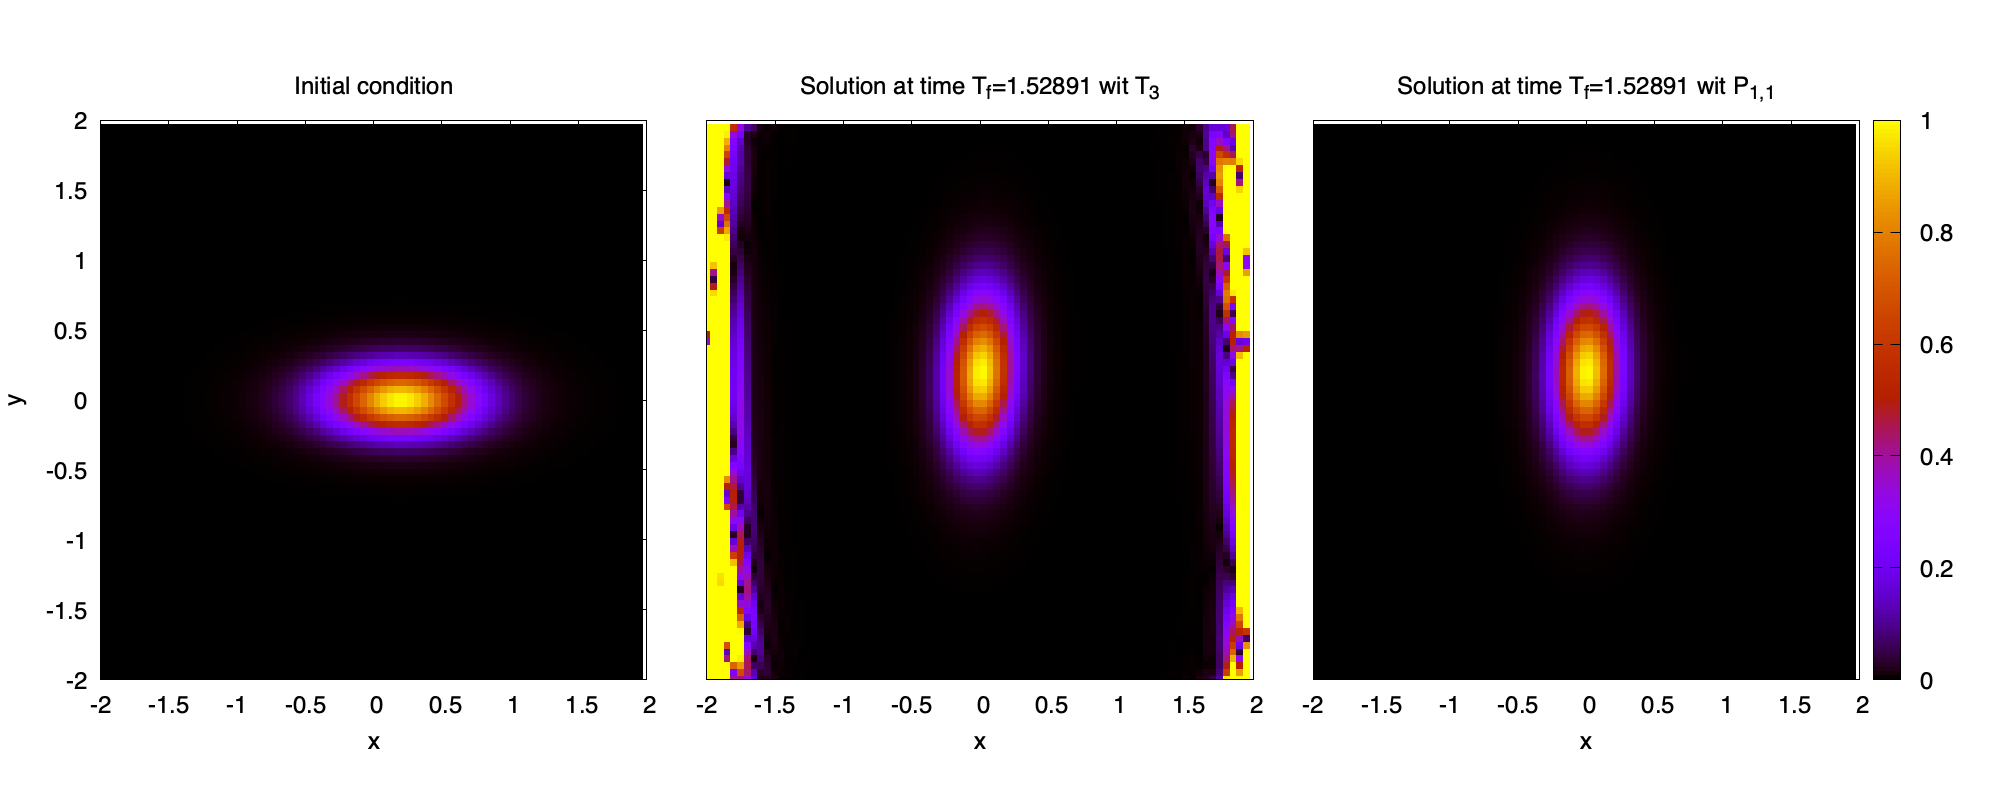
\includegraphics[width=\textwidth]{img/uf_t3p11}
    \caption{Initial condition (left), solution with Lawson RK(3,3) $T_3$ series (middle) and Lawson RK(3,3) $P_{1,1}$ approximant (right)}
  \end{figure}
\end{frame}

% -------------------------------------------------------------------
% --- NUMERICAL RESULTS ---------------------------------------------
% -------------------------------------------------------------------

\newcommand{\gz}{\textcolor{gris!80}{0}}

\section{Numerical results}
\begin{frame}{4D hybrid fluid-kinetic plasma model}
  Vlasov-Maxwell $1dz-3dv$ hybrid model
  \begin{itemize}
    \item Cold electrons \arrow fluid: cold current $(j_{c,x}(t,z),j_{c,y}(t,z))$
    \item Hot electrons \arrow kinetic: density in phase space $f_h(z,v_x,v_y,v_z)$
  \end{itemize}

  $$
    \partial_t U = LU + N(t,U)
  $$
  with $U = (j_{c,x},j_{c,y},B_x,B_y,E_x,E_y,f_h)^\top$ and
  $$
    L \!=\!\begin{pmatrix}
      \gz      & \!-\!B_0\! & \gz            &  \gz              &  \!\Omega_{pe}^2\! & \gz               & \gz \\ 
      \!B_0\!  &  \gz       & \gz            &  \gz              &  \gz               & \!\Omega_{pe}^2\! & \gz \\
      \gz      &  \gz       & \gz            &  \gz              &  \gz               & \partial_z        & \gz \\ 
      \gz      &  \gz       & \gz            &  \gz              & \!-\!\partial_z\!  & \gz               & \gz \\ 
      \!-\!1\! &  \gz       & \gz            & \!-\!\partial_z\! &  \gz               & \gz               & \gz \\ 
      \gz      & \!-\!1\!   & \!\partial_z\! &  \gz              &  \gz               & \gz               & \gz \\ 
      \gz      &  \gz       & \gz            &  \gz              &  \gz               & \gz               & \!\!\!\!\!-\!v_z\partial_z\! \\ 
    \end{pmatrix}
    ,\ 
    N\!:\!t,U\mapsto\!\begin{pmatrix}
      \gz \\
      \gz \\
      \gz \\
      \gz \\
      \int v_xf_h\dd{\Mvb{v}} \\
      \int v_yf_h\dd{\Mvb{v}} \\
      (\Mvb{E}\!+\!\Mvb{v}\times\Mvb{B})\!\cdot\!\nabla_{\!\Mvb{v}}f_h
    \end{pmatrix}
  $$
  \xmark can't compute $e^{tL}$ formally \hfill \cmark $P_{p,p}(tL)$ Padé approximant!
\end{frame}
\begin{frame}{Simulation code}
  We compare on this model:
  \begin{itemize}
    \item Strang \emph{classical} method, based on Hamiltonian splitting: order 2
    \item Lawson RK(4,4) classical (but some terms added in nonlinear term: Maxwell equations): order 4
    \item Lawson RK(4,4) with Padé $P_{2,2}$ approximant: order 4
    \item Lawson DP4(3) with Padé $P_{2,2}$ approximant: adaptive time step method
  \end{itemize}
  \mbold{Implementation details:}

  Problem with 7 variables, Padé approximant implies huge rational functions (with invert of matrix), high order Lawson methods have a lot of coefficients\dots Code generation \cmark
\end{frame}

\begin{frame}{Main idea of adaptive time step methods (error estimate)}
  for a generic ODE $\dot{u} = f(t,u)$, adaptive time step method need 2 numerical estimations of solution $u(t^{n+1})$ of different order, $p$ and $p+1$:
  $$
    u^{n+1}_{[p]} = u(t^{n+1}) + \order{\Delta t^{p+1}},\qquad u^{n+1}_{[p+1]} = u(t^{n+1}) + \order{\Delta t^{p+2}}
  $$
  Estimate of local error:
  \vspace{-0.5cm}
  $$
    L_{[p]}^{n+1} = \left| u^{n+1}_{[p+1]} - u^{n+1}_{[p]} \right|
  $$
  \mbold{If $L^{n+1}_{[p]}>tol$:} we reject the step and start again from time $t^n$. \mbold{Else} we accept the step. \mbold{In both cases}, the optimal new time step is:
  $$
    \Delta t_\text{opt} = \sqrt[p]{\frac{tol}{L^{n+1}_{[p]}}}\Delta t^n
  $$
  In practice $u^{n+1}_{[p]}$ is computed from sub-steps of $u^{n+1}_{[p+1]}$.

  \begin{thebibliography}{9}
    \setbeamertemplate{bibliography item}[article]
    \bibitem{g} \customcite{Dormand:1978} \textcolor{defaultcolor}{(for RK method)}
  \end{thebibliography}
  %In practice we don't want volatile time step:
  %$
  %  \Delta t^{n+1} = \max\left( 0.5\Delta t^n , \min\left( 2\Delta t^n , \Delta t_\text{opt} \right) \right)
  %$
\end{frame}

\begin{frame}{Numerical results}
  {$N_z\times N_{v_x} \times N_{v_y} \times N_{v_z} = 27 \times 32 \times 32 \times 41$}

  \only<1>{
    \begin{figure}
      \centering
      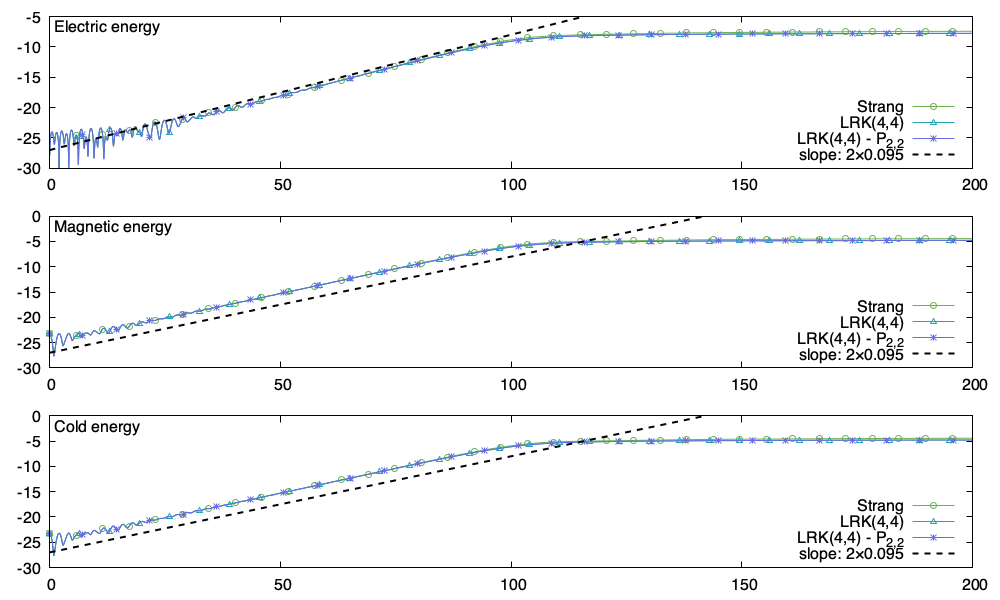
\includegraphics[width=0.93\textwidth]{img/energy_slrkp}
      \caption{Energies evolution for Strang, LRK(4,4) and LRK(4,4)-$P_{2,2}$ methods}
    \end{figure}
  }
  \only<2>{
    \begin{figure}
      \centering
      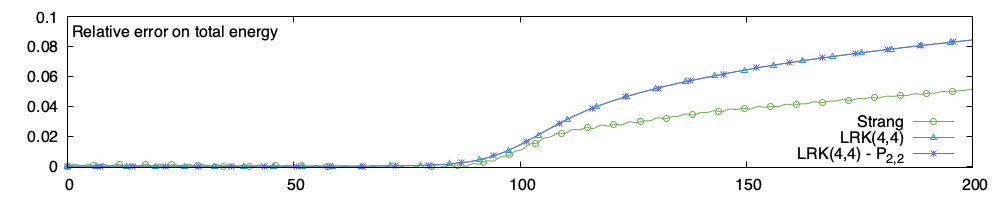
\includegraphics[width=0.93\textwidth]{img/error_slrkp}
      \caption{Relative error on total energy for Strang, LRK(4,4) and LRK(4,4)-$P_{2,2}$ methods}
    \end{figure}
  }
  \only<3>{
    \begin{figure}
      \centering
      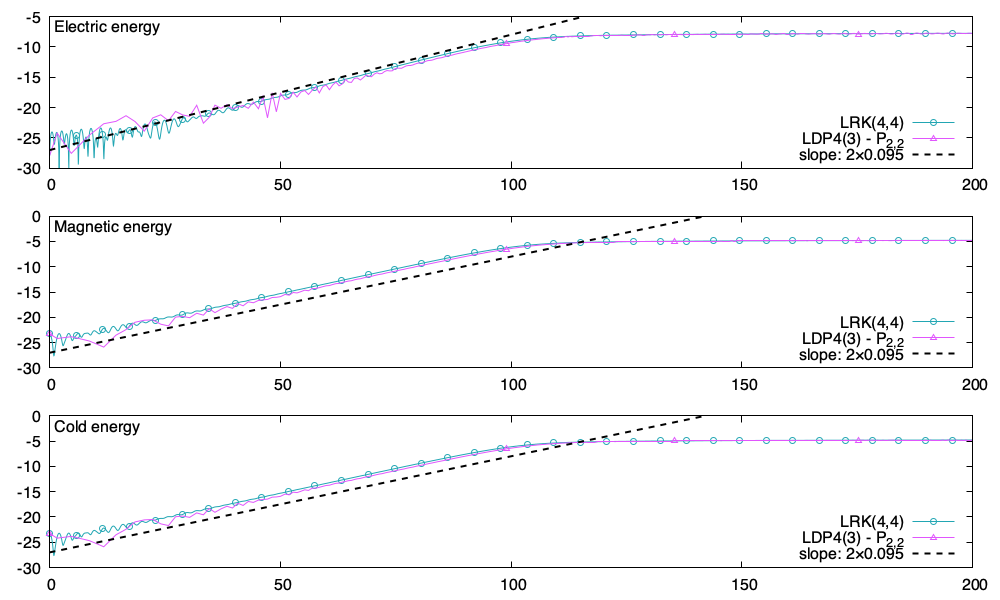
\includegraphics[width=0.93\textwidth]{img/energy_lrkdpp}
      \caption{Energies evolution for LDP4(3)-$P_{2,2}$ method}
    \end{figure}
  }
  \only<4>{
    \begin{figure}
      \centering
      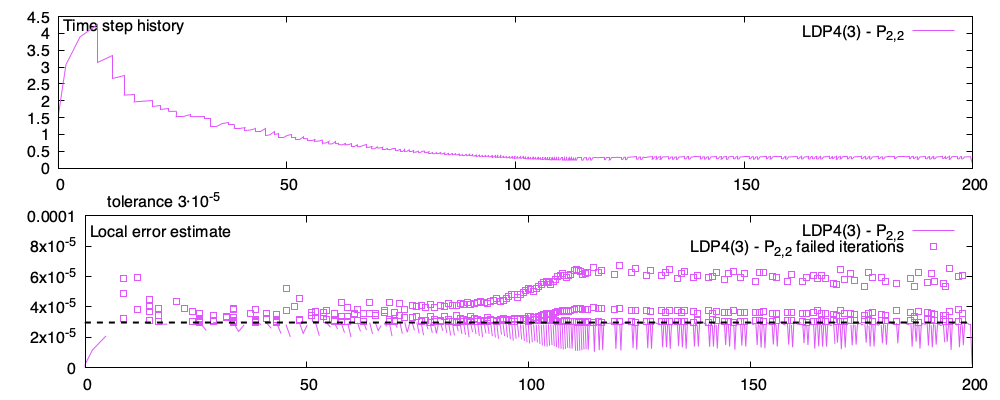
\includegraphics[width=0.93\textwidth]{img/dt_ldp43}
      \caption{Time step and estimate of local error evolution for LDP4(3)-$P_{2,2}$ method}
    \end{figure}
  }
\end{frame}

\begin{frame}{Simulation time}
  \begin{table}[h]
    \centering
    \begin{tabular}{l|r}
      time integrator & simulation time \\
      \hline
      Strang splitting     &    \textcolor{red}{$17\,\text{h}\ 09\,\text{min}\ 54\,\text{s}$} \\
      \hline
      LRK(4,4)             &                    $14\,\text{h}\ 06\,\text{min}\ 15\,\text{s}$ \\
      LRK(4,4) - $P_{2,2}$ &                    $13\,\text{h}\ 59\,\text{min}\ 59\,\text{s}$ \\
      \hline
      LDP4(3) - $P_{2,2}$  & \textcolor{mgreen}{$04\,\text{h}\ 09\,\text{min}\ 44\,\text{s}$} \\
    \end{tabular}
    \caption{Simulation time for some simulation, on mesh $N_z \times N_{v_x} \times N_{v_y} \times N_{v_z}=27\times32\times32\times41$ and time step $\Delta t = 0.05$ (initial time step for adaptive time step strategy).}
  \end{table}
\end{frame}

% -------------------------------------------------------------------
% --- CONCLUSION ----------------------------------------------------
% -------------------------------------------------------------------
\section{Conclusion}
\begin{frame}{Conclusion}
  \mbold{Conclusion:}
  \begin{description}
    \item[\xmark] Numerical cost of Hamiltonian splitting methods (not bad in $1dx-1dv$ but very bad in $1dz-3dv$, must be very very very bad in $3dx-3dv$ case)
    \item[\cmark] Numercial cost of Lawson methods
    \item[\bmark] Behavior of total energy of Lawson method (but we can use high order method easily)
    \item[\cmark] Error of approximation with Padé approximant can be lower than time integrator
    \item[\cmark] Very efficient adaptive time step method with computation of $e^{\tau L}$ with Padé approximant (more thinks can be in linear part)
  \end{description}
  \mbold{Future works}
  \begin{itemize}
    \item Add $\int \Mvb{v}f_h\dd{\Mvb{v}}$ in linear part (for $1dx-1dv$ Vlasov-Ampère model)
  \end{itemize}
\end{frame}

% -------------------------------------------------------------------
% --- THANKS --------------------------------------------------------
% -------------------------------------------------------------------
\begin{frame}[t]
  \vfill
  {\usebeamerfont{title} Thank you for your attention}
  \vfill
\end{frame}

\end{document}

